\section{inode Strukturreferenz}
\label{structinode}\index{inode@{inode}}
{\tt \#include $<$hashtab.h$>$}

Zusammengeh\"{o}rigkeiten von inode:\begin{figure}[H]
\begin{center}
\leavevmode
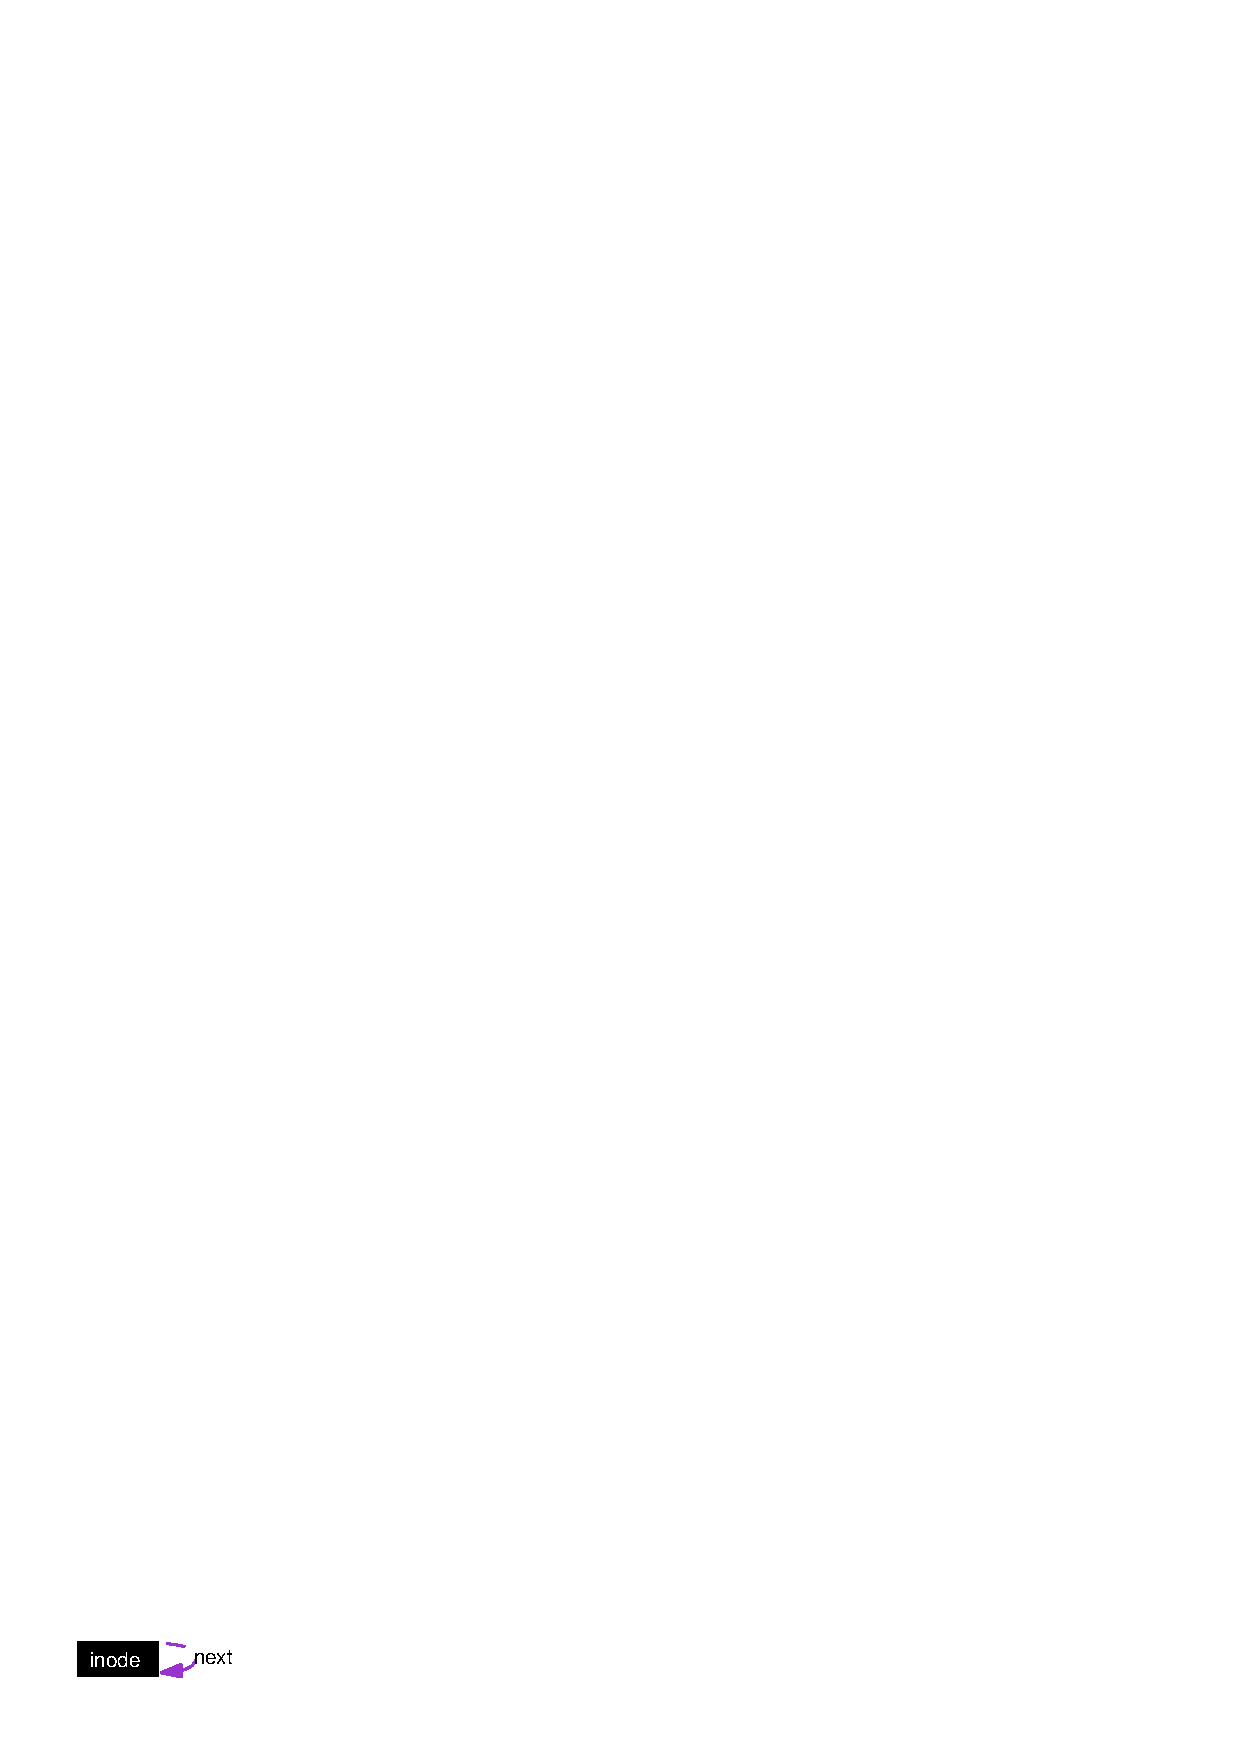
\includegraphics[width=57pt]{structinode__coll__graph}
\end{center}
\end{figure}
\subsection*{Datenfelder}
\begin{CompactItemize}
\item 
char $\ast$ {\bf string}
\item 
int {\bf flag}
\item 
u\_\-long {\bf count}
\item 
u\_\-long {\bf files}
\item 
u\_\-long {\bf visit}
\item 
u\_\-long {\bf tstamp}
\item 
double {\bf xfer}
\item 
{\bf inode} $\ast$ {\bf next}
\end{CompactItemize}


\subsection{Ausf\"{u}hrliche Beschreibung}




Definiert in Zeile 59 der Datei hashtab.h.

\subsection{Dokumentation der Datenelemente}
\index{inode@{inode}!count@{count}}
\index{count@{count}!inode@{inode}}
\subsubsection{\setlength{\rightskip}{0pt plus 5cm}u\_\-long {\bf inode::count}}\label{structinode_8579979bc170cd8cceafabe3208cfb3c}




Definiert in Zeile 61 der Datei hashtab.h.

Wird benutzt von all\_\-users\_\-page(), dump\_\-all\_\-users(), put\_\-inode() und top\_\-users\_\-table().\index{inode@{inode}!files@{files}}
\index{files@{files}!inode@{inode}}
\subsubsection{\setlength{\rightskip}{0pt plus 5cm}u\_\-long {\bf inode::files}}\label{structinode_16b7ee518b4af2b7cf436840aff1cc8c}




Definiert in Zeile 62 der Datei hashtab.h.

Wird benutzt von all\_\-users\_\-page(), dump\_\-all\_\-users(), put\_\-inode() und top\_\-users\_\-table().\index{inode@{inode}!flag@{flag}}
\index{flag@{flag}!inode@{inode}}
\subsubsection{\setlength{\rightskip}{0pt plus 5cm}int {\bf inode::flag}}\label{structinode_86565f81a8353154619812e7317b1e2d}




Definiert in Zeile 60 der Datei hashtab.h.

Wird benutzt von all\_\-users\_\-page(), dump\_\-all\_\-users(), put\_\-inode() und top\_\-users\_\-table().\index{inode@{inode}!next@{next}}
\index{next@{next}!inode@{inode}}
\subsubsection{\setlength{\rightskip}{0pt plus 5cm}struct {\bf inode}$\ast$ {\bf inode::next}}\label{structinode_ff3eec0bab3bda5c998d29251bb4d877}




Definiert in Zeile 66 der Datei hashtab.h.

Wird benutzt von del\_\-ilist(), load\_\-ident\_\-array() und put\_\-inode().\index{inode@{inode}!string@{string}}
\index{string@{string}!inode@{inode}}
\subsubsection{\setlength{\rightskip}{0pt plus 5cm}char$\ast$ {\bf inode::string}}\label{structinode_5883f2056e6f135990b1ba4be0d6017c}




Definiert in Zeile 59 der Datei hashtab.h.

Wird benutzt von all\_\-users\_\-page(), del\_\-ilist(), dump\_\-all\_\-users(), new\_\-inode(), put\_\-inode() und top\_\-users\_\-table().\index{inode@{inode}!tstamp@{tstamp}}
\index{tstamp@{tstamp}!inode@{inode}}
\subsubsection{\setlength{\rightskip}{0pt plus 5cm}u\_\-long {\bf inode::tstamp}}\label{structinode_737deeb7e731e4f9db70427fd0854dfd}




Definiert in Zeile 64 der Datei hashtab.h.

Wird benutzt von new\_\-inode() und put\_\-inode().\index{inode@{inode}!visit@{visit}}
\index{visit@{visit}!inode@{inode}}
\subsubsection{\setlength{\rightskip}{0pt plus 5cm}u\_\-long {\bf inode::visit}}\label{structinode_23fbc8ae83e74cc1ba882eef7b2a6948}




Definiert in Zeile 63 der Datei hashtab.h.

Wird benutzt von all\_\-users\_\-page(), dump\_\-all\_\-users(), new\_\-inode(), put\_\-inode() und top\_\-users\_\-table().\index{inode@{inode}!xfer@{xfer}}
\index{xfer@{xfer}!inode@{inode}}
\subsubsection{\setlength{\rightskip}{0pt plus 5cm}double {\bf inode::xfer}}\label{structinode_a3dee5fe9d1b73fa4dfffc800e8a3cdf}




Definiert in Zeile 65 der Datei hashtab.h.

Wird benutzt von all\_\-users\_\-page(), dump\_\-all\_\-users(), put\_\-inode() und top\_\-users\_\-table().

Die Dokumentation f\"{u}r diese Struktur wurde erzeugt aufgrund der Datei:\begin{CompactItemize}
\item 
oosalizer/{\bf hashtab.h}\end{CompactItemize}
